\section{Labeling Module}
\label{sec:labeling}
Labeling module manages one RIB-IN table associated with a peer if configured and uses the tables to assign labels to updates received from the peer.  In this module, the only configuration is about how to process the BGP updates from peers. It is specified by "labelAction" in peer configuration as shown in Figure \ref{fig:configurationSub}. "labelAction" could be one of these three options:
\begin{itemize}
\item{ \emph{None:} Don't process the updates at all. }
\item{ \emph{RibStore:} Store the updates in RIB-IN tables on a per-peer basis. The peer has its own RIB-IN table if this option is set.}
\item{ \emph{Label:} Store the updates in RIB-IN tables and label the updates based on how they change RIB-IN tables. This option implicitly stores RIB-IN for the peer. }
\end{itemize}
Since the RIB-IN tables are the major memory consumption of BGPmon, one might want to set "labelAction" as "None" if the memory is the major concern. 

Labeling module has a single thread which is a reader of peer queue and a writer of label queue as shown in Figure \ref{fig:architecture}. Main flow has three steps:
\begin{itemize}
\item{ Read the BMF messages from peer queue }
\item{ If the BMF message is a update, then process it based on the "labelAction" configuration. Otherwise, do nothing.}
\item{ Write the processed BMF messages into labeling queue }
\end{itemize}
The detail of main flow logic will be discussed in section \ref{sec:labeling:mainflow}.

\subsection{Data Structure}
Labeling Module uses 2 main data structures(PrefixTable and AttrTable) to maintain the RIB-IN table. As the RIB-IN table is maintained on a per-peer basis, it is natural to make these 2 structures as components of the "Session" structure as we mentioned in section \ref{sec:peering:sessionstructure}.  "PrefixTable" and "AttrTable" are used to store prefixes and attributes in BGP updates respectively. And these 2 tables are inter-linked to make up one RIB-IN table.

\subsubsection{ PrefixTable Structure}
\label{sec:labeling:prefixtable}
In our design it is a hash table that consists of multiple entries. Each entry is a link list of nodes and each node contains a prefix. It has the following six parts.
\begin{itemize}
\item{\emph{prefixCount:} is the number of prefixes are contained in the prefix hash table.}
\item{\emph{tableSize:} is the number of entries in the hash table.}
\item{\emph{occupiedSize:} is the number of occupied entries in the hash table. Occupied entry means it has at least one node. }
\item{\emph{maxNodeCount:} is the max length among all entries in the hash table. The length of one entry indicates how many nodes it contains.}
\item{\emph{maxCollision:} is the max number of nodes one entry is allowed to contain. If one entry contains too many nodes, we need to increase the number of entries in a hash table in order to improve the performance. Basically if maxNodeCount is larger than maxCollision, we need to enlarge the hash table.}
\item{emph{prefixEntries:} is an array of PrefixEntry structures. It contains all the entries of the prefix hash table. For the details of PrefixEntry structure, see Figure \ref{fig:PrefixEntryStruct}.}
\end{itemize}
\begin{figure*}
\centering
\scalebox{0.8}{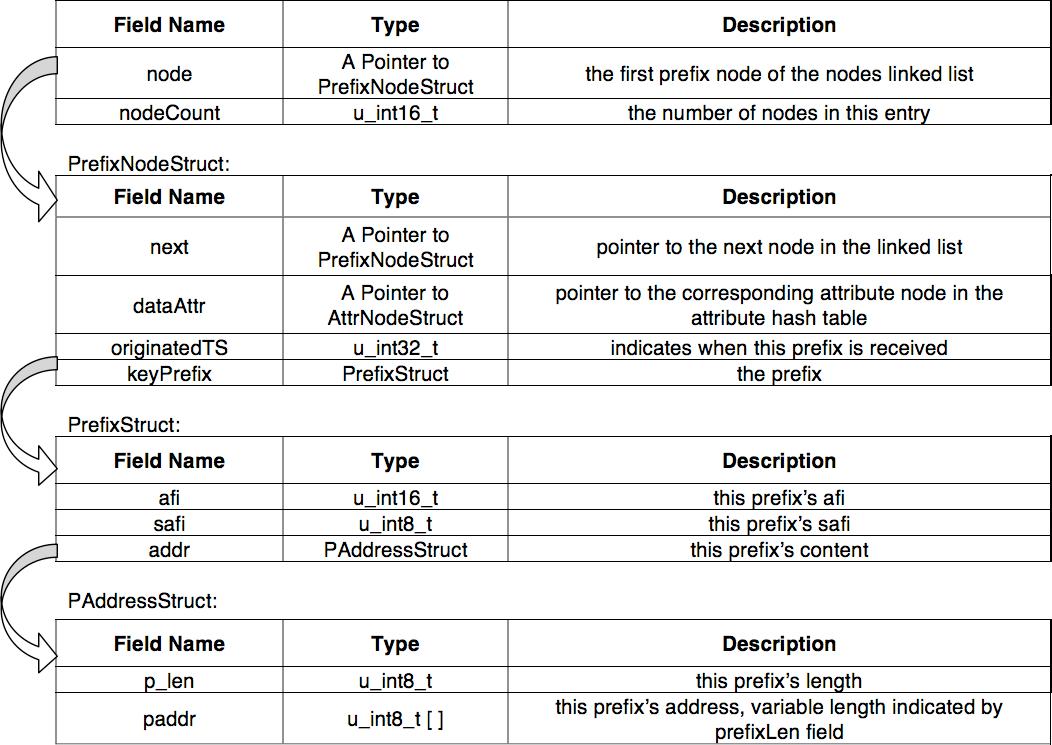
\includegraphics{figs/PrefixEntryStruct.pdf}}
\caption{PrefixEntry Structure}
\label{fig:PrefixEntryStruct}
\end{figure*}
Each prefix in the NLRI of a BGP update will be one node of a particular entry in the prefix table. The index of this entry is calculated by hash value of the prefix. 
2 same prefixes will be hashed to the same entry and stored in the same node.
Because of hash collision, 2 different prefixes could also be hashed to the same entry. But they will be stored in difference nodes of this entry.

\subsubsection{AttributeTable Structure}
\label{sec:labeling:attributetable}
Attribute hash table is similar to the prefix hash table mentioned in the previous section. AttributeTable structure is used to implement a hash table to store the attributes of BGP updates. It has the following six parts.
\begin{itemize}
\item{\emph{attributeCount:} is the number of attributes are contained in the attribute hash table.}
\item{\emph{tableSize:} is the number of entries in the hash table.}
\item{\emph{occupiedSize:} is the number of occupied entries in the hash table. }
\item{\emph{maxNodeCount:} is the max length of all entries in the hash table.}
\item{\emph{maxCollision:} is the max number of nodes one entry is allowed to contain.}
\item{\emph{attrEntries:} is an array of AttrEntry structures. For the details of AttrEntry structure, see Figure \ref{fig:AttributeEntryStruct}.}
\end{itemize}
\begin{figure*}
\centering
\scalebox{1}{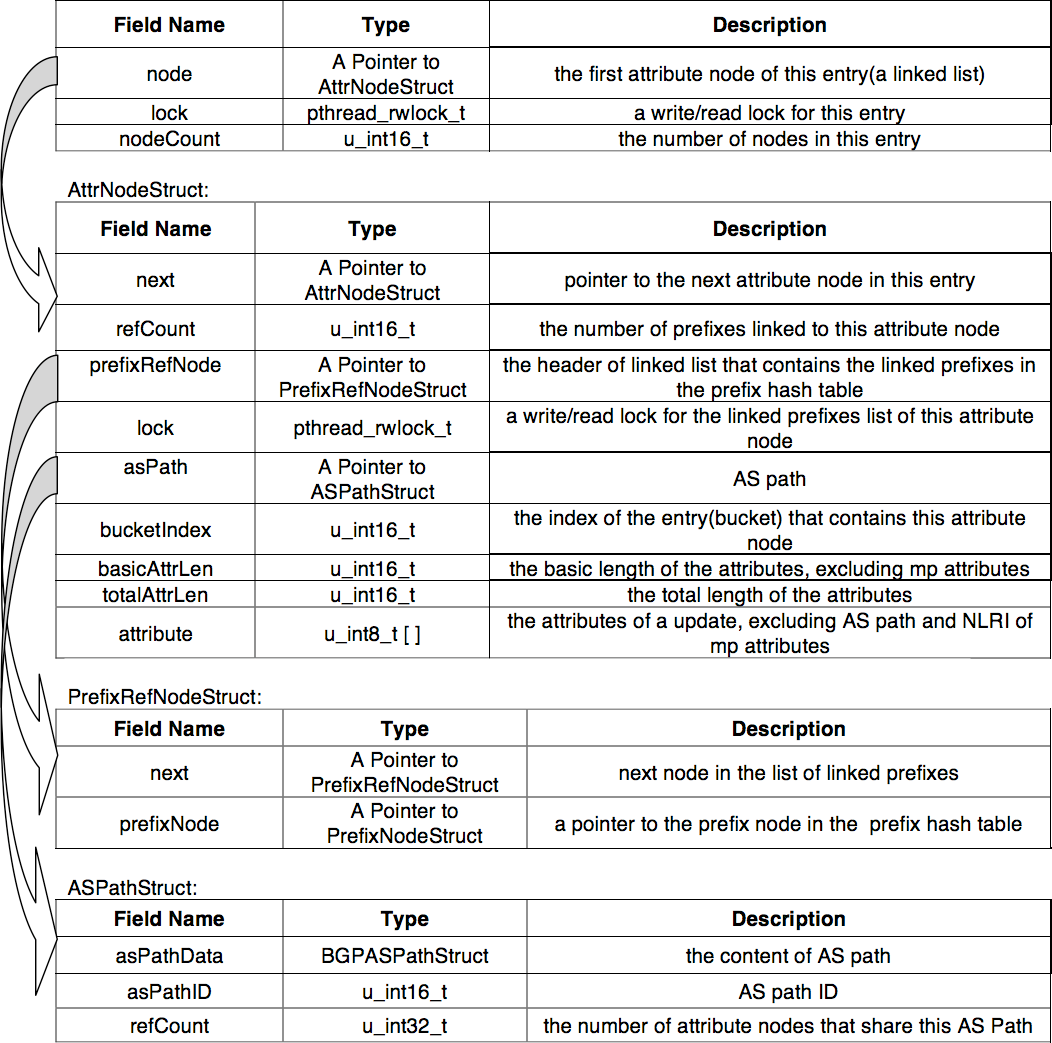
\includegraphics{figs/AttributeEntryStruct.pdf}}
\caption{AttributeEntry Structure}
\label{fig:AttributeEntryStruct}
\end{figure*}
In the attribute table, the attribute set in a BGP update will be stored in one node. And which entry this node belongs to is determined only by the hash value of AS path.
That means if 2 attribute sets have the same AS path, they will be hashed to the same entry. If other attributes of the 2 sets are also same, they will be stored in the same node. 
If 2 attribute sets have the same AS path but other attributes are different, they will still be stored in the same entry but 2 different nodes.  
Note in the case the AS path is only stored once and the 2 different nodes will link to the same AS path.
Again it is possible that  2 attribute sets with different AS paths are hashed to the same entry because of hash collision.

   

\subsection{Main Flow Logic}
\label{sec:labeling:mainflow}
After introducing the data structure, we describe the main flow logic of labeling module here. As we mentioned, labeling module reads the BMF messages from peer queue. For the BMF messages with type other than 2 (see Figure \ref{tab:types}), the labeling module simply writes them into labeling queue without any processing.  For each BMF message with type 2, labeling module processes it as follows:  
\begin{itemize}
\item{If it doesn't contain a BGP update message, simply writes it into labeling queue without any processing.}
\item{If it contains a BGP update message,  extract the session ID from the BMF message. With the sesionID the labeling module finds the peering session structure and checks the 'labelAction' in it (see Figure \ref{fig:configurationSub}).  }
	\begin{itemize}
		\item{If the field 'labelAction' is set to "None", simply writes the BMF message into label queue without any processing.}
		\item{If the field 'labelAction' is set to "RibStore", updates the RIB-IN table of the corresponding peering session and then writes the the BMF message into label queue. In section \ref{sec:labeling:storerib} we will discuss the detail about how to update RIB-IN tables given a BGP update message. }
			\item{If the field 'labelAction' is set to "label", updates the RIB-IN table of the corresponding peering session and labels this BMF message. Specifically, one label for each prefix in NLRI will be attached to the BMF message and its message type will be changed to 3. Finally the new BMF message with type 3 will be written into label queue. In section \ref{sec:labeling:label} we will discuss the detail about how to label a BGP update message.}
	\end{itemize}
\end{itemize}

\subsection{Store RIB-IN Tables}
\label{sec:labeling:storerib}
The labeling module stores RIB-IN tables on a per-peer basis. For each incoming BGP update message from a peer, the labeling module stores it in the peer's RIB-IN table as follows:
\begin{enumerate}
	\item{Parse the BGP update message into the following components:}
	\begin{itemize}
		\item{IPv4 unicast reachable NLRI and unreach NLRI}
		\item{multiple protocol(mp) reachable NLRI and unreach NLRI}
		\item{the attribute set excluding AS path, mp unreachable attributes and NLRI of mp reachable attributes}
		\item{AS path}
	\end{itemize}
	
	\item{Hash the AS path and find the entry in the attribute table based on the hash value. Then check each node of this entry against the AS path and attribute set from above as follows:}
	\begin{itemize}
		\item{If the current node's AS path and attribute set are the same, return this attribute node.}
		\item{If the current node's AS path is same but attribute set is not, return a new created attribute node that has the new attribute set and is linked to the existing AS path. Recall the same AS path shared by multiple nodes is only stored once.}
	\end{itemize}
	\item{If none of the nodes matches the above 2 rules, return a new created attribute node with the new AS path and attribute set.}
		
	\item{Extract all prefixes from IPv4 unicast reachable NLRI and mp reachable NLRI. Each prefix is processed as follows: }
	\begin{itemize}
		\item{If there is a existing prefix node which contains the same prefix content such as such as afi, safi, mask length and address in the prefix hash table:}
		\begin{itemize}
			\item{If the existing prefix node's linked attribute node('dataAttr' field in Figure\ref{fig:PrefixEntryStruct}) is same as the attribute node returned from step 2, do nothing.}			\item{Otherwise:}
			\begin{itemize}
				\item{Delete this prefix node from its current attribute node's linked prefix nodes list. If there isn't any prefix node linked to this attribute node after this deletion, remove this attribute node from the attribute hash table.}
			\item{Add this prefix node to the linked prefix nodes list in the attribute node returned from step 2.}
			\end{itemize} 	
		\end{itemize}
		\item{Otherwise:}
		\begin{itemize}
			\item{Create a prefix node(PrefixNodeStruct, see Figure\ref{fig:PrefixEntryStruct}) based on the prefix's content.}
			\item{The created prefix node is placed into an entry(PrefixEntryStruct, see Figure\ref{fig:PrefixEntryStruct}) in the prefix hash table based on the hash value of the prefix's content.} 			\item{Update its linked attribute node field('dataAttr' field in Figure\ref{fig:PrefixEntryStruct} with the attribute node returned from step 2. }
			\item{As each attribute node maintains a list of all linked prefix nodes, we also need to add this new created prefix node to that list of the attribute node returned from step 2}
		\end{itemize}
	\end{itemize}
	
	\item{Extract all prefixes from the IPv4 unicast unreachable NLRI and multiprotocol unreachable NLRI. Each prefix is processed as follows:}
	\begin{itemize}
		\item{If there is a existing prefix node which contains the same prefix content such as such as afi, safi, mask length and address in the prefix hash table:}
		\begin{itemize}
			\item{Delete this prefix node from its corresponding attribute node's linked prefix nodes list. If there isn't any prefix node linked to this attribute node after this deletion, remove this attribute node from the attribute hash table.}
			\item{Remove this prefix node from the prefix hash table.} 		\end{itemize} 					
		\item{Otherwise: Do nothing.}
	\end{itemize}		
\end{enumerate}


\subsection{Labels the BGP updates}
\label{sec:labeling:label}
The labeling module labels all the prefixes in a BGP update message base on how they change RIB-IN tables. More specifically, the label classifies the prefixes into six categories: 'new announcement' versus 'duplicate announcement', 'same path' versus 'different path' and 'withdraw' versus 'duplicate withdrawal'. In BGP one update consists of multiple prefixes which share the same set of attributes and these prefixes might change the RIB-IN tables in different ways. As a result, the multiple prefixes in one BGP updates have to be labeled separately. That's why labeling has to be done on a per-prefix basis, not a per-update basis.

Labeling is done as follows:
\begin{enumerate}
	\item{Return a existing or new created attribute node according the step 1 and 2 in the preview subsection. }
	\item{Extract all prefixes from IPv4 unicast reachable NLRI and multiprotocol reachable NLRI. Each prefix is labeled as follows: }
	\begin{itemize}
		\item{If there is a existing prefix node which contains the same prefix content such as such as afi, safi, mask length and address in the prefix hash table:}
		\begin{itemize}
			\item{If the existing prefix node's linked attribute node ('attributeNode' field in Figure\ref{fig:PrefixEntryStruct} is same as the attribute node return from step 1, label it as 'duplicate announcement'.}			\item{Otherwise, compare the 'AS Path' in this prefix node's current linked attribute node to the 'AS Path' in the attribute node returned from step 1. }
			\begin{itemize}
				\item{If they are same, label it as 'same path'. }				\item{Otherwise, label it as 'different path'. }
			\end{itemize} 	
		\end{itemize}			    
		\item{Otherwise, label it as 'new announcement'. }
	\end{itemize}
	
	\item{Extract the IPv4 unicast unreachable NLRI and multiprotocol unreachable NLRI. Each prefix is labeled as follows:}
	\begin{itemize}
		\item{If there is a existing prefix node which contains the same prefix content such as such as afi, safi, mask length and address in the prefix hash table, label it as 'withdraw'}		
			\item{Otherwise:  label it as 'duplicate withdraw'.}
	\end{itemize}
\end{enumerate}
	
\subsection{Design Philosophy}
The first design issue here is how to organize a RIB table in memory. Logically a RIB table can be viewed as prefixes and attributes that are interlinked together. And another observation is that a set of attributes is typically shared by multiple prefixes as they are received in one BGP update.  Based on these observations. we decided to store a RIB by using 2 interlinked hash tables: prefix hash table and attribute hash table.
As we discussed in subsecions \ref{sec:labeling:prefixtable} and \ref{sec:labeling:attributetable}, these 2 hash tables has the same structure in a high level. Specifically both of them consists of multiple entries and each entry is a linked list that has multiple nodes. In the prefix hash table each node represents a prefix and in attribute hash table each node holds a set of attributes. And the prefixes and the set of attributes are linked together if they are received in the same BGP update. Note one prefix node representing a single prefix can only be linked to one attribute node holding a set of attributes. But one attribute node could be linked to multiple prefix nodes. In other words, the relationship between prefix node and attribute node is many to one.

The second design issue is how to store the prefixes and the set of attributes in a BGP update efficiently. For a prefix it is straightforward to hash the prefix to an entry(bucket) in the prefix hash table. Then all the nodes of this entry are checked in order to know if this prefix is existing or not. For the set of attributes, we have 2 options here:
	\begin{itemize}
		\item{\emph{Option1: }Hash the entire set of attributes to an entry of attribute hash table.}		
		\item{\emph{Option2: }Extract the AS path form the set of attributes and then hash the AS path to find an entry for the set of attributes.}
	\end{itemize}
Each option has its own pros and cons. Option1 basically hashes each unique set of attributes to a different entry(bucket) if ignoring the hash collision. That will make the attribute hash table too long in terms of the number of entries.
In option2 each set of attributes is assigned to a entry based on the hash value of its AS path. The implication is that all sets of attributes with the same AS path will be assigned to the same entry. As a result, option2 will take fewer entries than needed by option1. But each entry will have more nodes in option2 than option1. So it is a tradeoff between the number of entries and the length of entries.

But besides that option2 is better in comparing the AS paths in 2 sets of attributes. In option2 2 sets of attributes that have different AS paths must be assigned to the different entry. But  2 sets of attributes assigned to the same entry don't necessarily have the same AS path because of hash collision. So when attribute node gets created we tag its AS path with ID in order to differentiate the different AS paths that are assigned to the same entry because of hash collision. As a result, we can compare the AS paths in 2 sets of attributes as follows:
	\begin{itemize}
		\item{If they are assigned to different entries, we know they have different AS paths.}
		     \item{If they are assigned to the same entry, continue to compare their AS Paths' IDs.}
		\begin{itemize}
			\item{If they are the same, we know they have the same AS path.}			
				\item{Otherwise, we know they have different AS paths.}
		\end{itemize}
	\end{itemize}
Contrast to option2, comparing the AS paths in 2 sets of attributes would be more complex in option1 because one first needs to extract the 2 AS paths from them then compare the 2 AS paths in bitwise. That could be a big flaw of option1 as this operation is done for every receiving prefix in BGPmon.

Another advantage of option2 is that all the sets of attributes have the same AS path will share the same AS path structure in memory. In option1 each set of attributes stores the AS path respectively even some of them have the same AS path. So option2 is also better in terms of memory consumption.
Based on all of these, we decided to use option2 in our current design.
 
The last design issue here is about configuration changes. As we mentioned, the only related configure item here is "labelAction" which has 3 values: None, RibStore and Label. All the possible changes are listed:
\begin{itemize}
\item{If "labelAction" changes from Label to RibStore, nothing needs to be done. The labeling module will automatically turn off the labeling fucntion.}
\item{If "labelAction" changes from RibStore to Label, nothing needs to be done. The labeling module will automatically turn on the labeling fucntion.}
\item{If "labelAction" changes from RibStore to None, the RIB table needs to be freed.}
\item{If "labelAction" changes from Label to None, the RIB table needs to be freed.} 
\item{If "labelAction" changes from None to Label, this change cannot be applied immediately. If we apply this change immediately, the labeling will misbehave as we don't have the RIB. For instance, right after the change all the updates labelled as 'new announcement' are actually not new. } 
\item{If "labelAction" changes from None to RibStore,  this change cannot be applied immediately either. If we start to store RIB immediately and right after that user further changes it from RibStore to Label, we will run into the same problem as above. } 
\end{itemize}
The only way to make the last 2 changes applied is to reset the session. When a new session starts, the changes will be applied automatically and labeling will behave correctly.
